\documentclass[9pt, oneside]{book}
\usepackage{xeCJK}
\usepackage{amsmath, amsthm, amssymb, bm, graphicx, hyperref, mathrsfs}
\usepackage{geometry}
% \geometry{b5paper,scale=0.85}
\geometry{a4paper,left=1.2cm,right=1.2cm,top=2cm,bottom=1cm}
\usepackage{graphicx} %插入图片的宏包
\usepackage{float} %设置图片浮动位置的宏包
\usepackage{subfigure} %插入多图时用子图显示的宏包
\usepackage{amstext} %公式中包含文字的宏包
\usepackage{booktabs} %插入表格的宏包
\usepackage{multirow} 
\usepackage{indentfirst} %设置缩进的宏包
\setlength{\parindent}{2em}
\usepackage{enumerate} %用于编号的宏包
\usepackage{hyperref} %用于引用的宏包
% \hypersetup{colorlinks, linkcolor=blue} %设置引用的字体颜色
\usepackage{color} %用于设置字体颜色的宏包
\usepackage{url} %用于超链接的宏包
\usepackage{bm} %用于公式加粗


% 封面部分
\title{\Huge{\textbf{自动飞行控制:原理与实务 \\ Notebook}}}
\author{Wu Yutian}
\date{2022.1.12}
\linespread{1.4}
\newtheorem{theorem}{定理}[section]
\newtheorem{definition}[theorem]{定义}
\newtheorem{lemma}[theorem]{引理}
\newtheorem{corollary}[theorem]{推论}
\newtheorem{example}[theorem]{例}
\newtheorem{proposition}[theorem]{命题}
\begin{document}

% 输出封面
\maketitle

% 前言部分
\pagenumbering{roman}
\setcounter{page}{1}

\begin{center}
    \Huge\textbf{前言}
\end{center}~\

~\\
\begin{flushright}     
    \begin{tabular}{c}
        Wu Yutian\\
        2022.1.12
    \end{tabular}
\end{flushright}

\newpage
\pagenumbering{Roman}
\setcounter{page}{1}
\tableofcontents
\newpage
\setcounter{page}{1}
\pagenumbering{arabic}

\chapter{航电系统介绍}

\section{航电系统的组成}

\subsection{航电系统的十大组成部分:}

\subsubsection{显示器(Display)}

\begin{itemize}
    \item [-] 抬头显示器(Head Up Display——HUD): \\ 
        为了让驾驶员在专注于机外世界时不必改变头的角度,就可以看到仪表上的重要信息,如武器的瞄准线和红外夜视仪的影像等.
    \item [-] 头盔显示器(Helmet Mounted Display——HMD): \\
        头盔显示器更能方便驾驶员随时观看到画面,红外夜视仪可能会放在头盔显示器上.
    \item [-] 低头显示器(Head Down Display——HDD): \\
        HDD就是一般的彩色多功能面板,它的信息也很重要,但是不需要驾驶员无时无刻注意.主要包括一些飞行状况(高度,空速,俯仰角等),导航状况(飞机位置,目的地位置等),飞机健康状况(引擎状态,电力供应等).
\end{itemize}

\subsubsection{通信系统(communication)}

通讯依频率不同可以分为以下几种:

\begin{itemize}
    \item [-] HF(High Frequency)通讯:范围在$2\sim 30MHz$之间,用于长距离通讯.
    \item [-] VHF(Very High Frequency)通讯:范围在$30\sim 100MHz$之间,用于中距离通讯.
    \item [-] UHF(Ultra High Frequency)通讯:范围在$250\sim 4500MHz$之间,为军用飞机频道.
    \item [-] SATCOM(Satellite Communication):可提供全球性的通讯管道.
\end{itemize}

通常一架飞机需要拥有两套以上的通讯系统,民航飞机由于安全性的考量,更配有三套通讯系统(redundancy-冗余).

\subsubsection{数据输入与控制(Data Entry and Control)}

驾驶员输入指令的方式:键盘输入,触摸式面板输入,语言输入.

\subsubsection{飞行控制系统(Flight Control System)}

飞控系统根据其执行的功能,可以分为两个层次:

\begin{itemize}
    \item [-] 增稳系统(Stability Augmentation): \\
        是针对稳定的飞机而控制.通常稳定型的飞机,即使显示元放开操纵杆,飞机仍会自行到达稳态,不过到达稳态的时间可能很长,而且飞机会有很大的振荡.增稳控制系统就是要协助飞机快速平顺地到达稳态.
    \item [-] 线控系统(Fly By Wire, FBW): \\
        对于先天性不稳定地飞机,如高性能战斗机,其重心在气动力中心地后方,只要驾驶员一松开操纵杆,机头即有向上翻仰地倾向,也就是说飞机随时都处于不稳定状态,需要电脑实时监控.线控飞机有别于传统飞机以驾驶员手直接拉连杆而移动控制翼面,它是由电脑送出指令,通过导线,驱动液压系统,再移动翼面,因此称之为线控. \\
        先天不稳定的飞机响应很快,若无电脑的帮助,人无法阻止飞机的发散行为.
\end{itemize}

\subsubsection{飞机状态感测系统(Aircraft State Sensor Systems)}

测量飞机状态的传感器可分为两大类:

\begin{itemize}
    \item [-] 空气数据系统(Air Data Systems): \\
        此系统测量飞机所在的大气环境,如风向,风速,大气压,高度等,这些大气环境的信息,都可以经过三个基本的量测值组合而成.这三个基本的量测值是:(1)静压力(Static Pressure).(2)全压力(Total Pressure).(3)大气温度.
    \item [-] 惯性感测系统(Interial Sensor Systems): \\
        此系统要测量飞机的位置和姿态相对于惯性坐标系的变换.惯性感测元件有陀螺仪(gyro)和加速度计(accelerometer).
\end{itemize}

\subsubsection{导航系统}

导航系统的目的在于告诉驾驶员现在飞机的位置,飞行的速度及方向,并能确认目的地在哪里,距离有多远,还要飞多久可以到达.导航系统有两种,一般的飞机兼具有两种功能:

\begin{itemize}
    \item [-] 推测领航(Dead Reckoning Navigation System): \\
        此种导航法是根据飞行速度估算出飞机相对于某一已知点的飞行距离,进而求出飞机现时的位置.一般来说有三种不同的推测领航系统,它们都可以独立操作,与地面站无关:
        \begin{itemize}
            \item 惯性导航系统: \\
                使用陀螺仪和加速度计测量角度和位置,准确度较高,被广泛应用.
            \item 多普勒方位参考系统: \\
                以多普勒位移原理(多普勒效应指出,波在波源移向观察者时接收频率变高,而在波源远离观察者时接收频率变低,这种位移现象称为多普勒位移.)\textcolor[rgb]{1,0,0}{(使用多普勒原理难道不是需要在地面上有一个波的接收机或者发射器吗?这还算是与地面站无关?)},测量速度和方位,常用于直升机\textcolor[rgb]{1,0,0}{(为什么常用于直升机,直升机的应用场景有什么特殊的地方么?)}
            \item 大气数据方位参考系统: \\
                此系统以大气环境的三个测量值反推非u及的飞行速度和方向,最为便宜,但精度也最差.
        \end{itemize}
        推测领航法的优点是独立运作,不受外界的干扰;缺点是位置估测误差会积累.
    \item [-] 无线电导航系统(Radio Navigation Systems):
        这类导航系统是借由飞机上的接收机,接收来自地面上塔台或者天上的人造卫星的信号.由于地面塔台或者天上的人造卫星的位置已知,因此可以根据所收到的无线电波的方位以及无线电波的传递时间,计算出飞机相对于信号发送源的距离和方向角.无线电导航系统有下面几种:
        \begin{itemize}
            \item [-] GPS(Global Position System):最精确的无线电导航系统.
            \item [-] VOR/DME:地面航站向四面八方发射VHF波段的无线电波,飞机根据接收到的无线电波的入射角以及到达时间,即可计算出飞机相对于地面航站的距离以及方向角.
            \item [-] LS/MLS:仪器降落与微波降落系统:是借由无线电波和微波导引飞机的降落,是属于近距离的导航.
        \end{itemize}
\end{itemize}

\subsubsection{机外环境感测系统(External World Sensor Systems)}

此感测系统包含雷达(radar)以及红外线感测仪(Ingrared Sensor)用以辅助飞机全天候,全天时的飞行能力.

\subsubsection{功能自动化系统(Task Automation Systems)}

此系统用于减轻驾驶员的飞行负担,减少所需要的机组人员,主要功能包括:

\begin{itemize}
    \item [-] 导航管理系统(Navigation Management System):自动处理来自INS(Inertial Navigation System)和GPS的信号,自动估计飞机现时状态,自动指示下一时刻的飞行方向.
    \item [-] 自动驾驶仪(Auto-pilot):实现定航向飞行,定高度飞行,定速飞行,陆地追随飞行(飞机可以贴着地面飞行,随着地表的高低起伏而飞上飞下,但和地面保持约$100\sim 200ft$的固定间隔)等.
    \item [-] 飞行管理系统(Flight Management System-FMS):执行飞行路劲规划,导航管理,引擎控制等功能.
    \item 
\end{itemize}

\subsubsection{引擎控制与管理(Engine Control and Management)}

\subsubsection{舱内常态管理(House Keeping Management)}

\section{航空电子的操作环境}

\section{国内航电系统发展趋势与市场分析}

\section{微软模拟飞行软件简介}


\chapter{飞行运动的描述}

本章介绍基本的飞机空气动力特性,飞机的稳定性及动态响应,以作为后续各章(线传飞行控制及自动驾驶仪)的学习基础

\section{机翼的特性与功能}

\subsection{机翼的几何外形}

如下图所示,我们先定义了翼面各部分的名称.翼展(span)的长度是垂直于机身的方向,从左翼尖量到右翼尖的长度.我们称翼展是在飞机的横方向,而翼弦长(chord)则是在飞机的纵方向.
\begin{figure}[H]
    \centering
    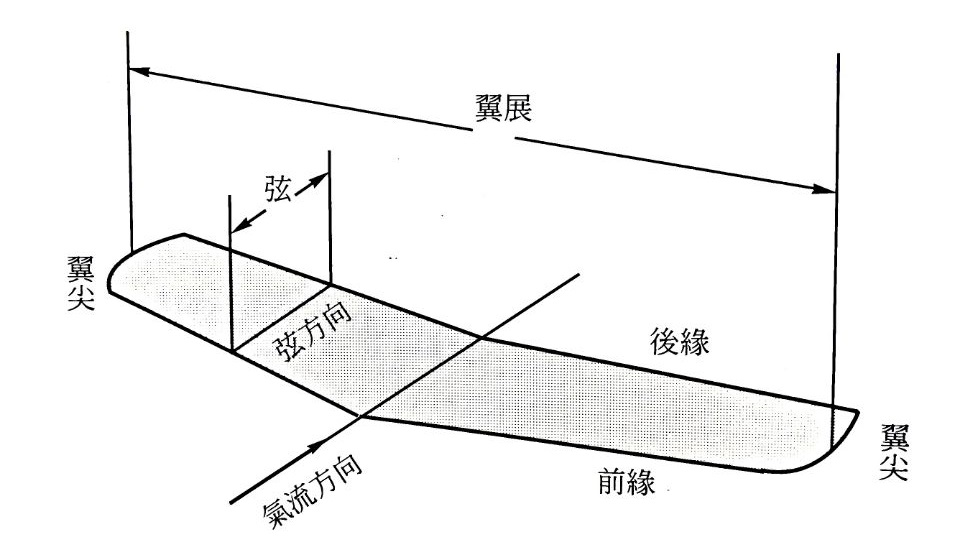
\includegraphics[width=0.5\linewidth]{image/2-1.jpg}
\end{figure}

另外,飞机的左右两翼并非水平的安置在机身上,这个往上翘的角度称为上反角,如下图所示.
\begin{figure}[H]
    \centering
    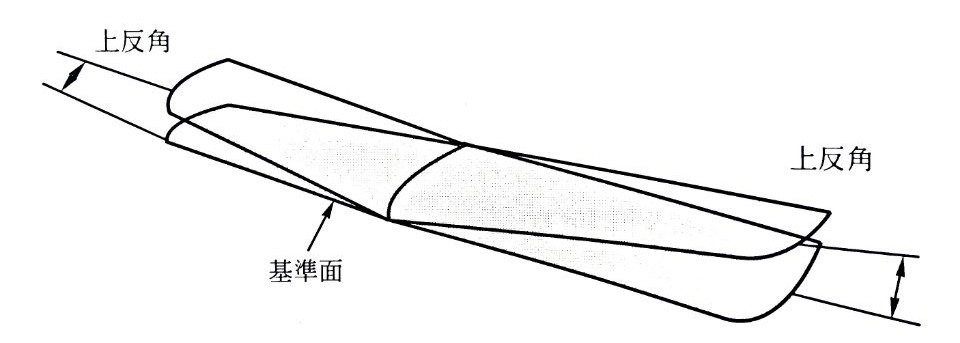
\includegraphics[width=0.6\linewidth]{image/2-2.jpg}
\end{figure}

机翼的中心线和机身的中心线并不平行,因此机身水平前进时,机翼和相对风之间存在一个夹角,称为攻角,如上图所示.这一夹角使得机头不必抬起,机身就可以获得足够的升力以抵抗重力.
\begin{figure}[H]
    \centering
    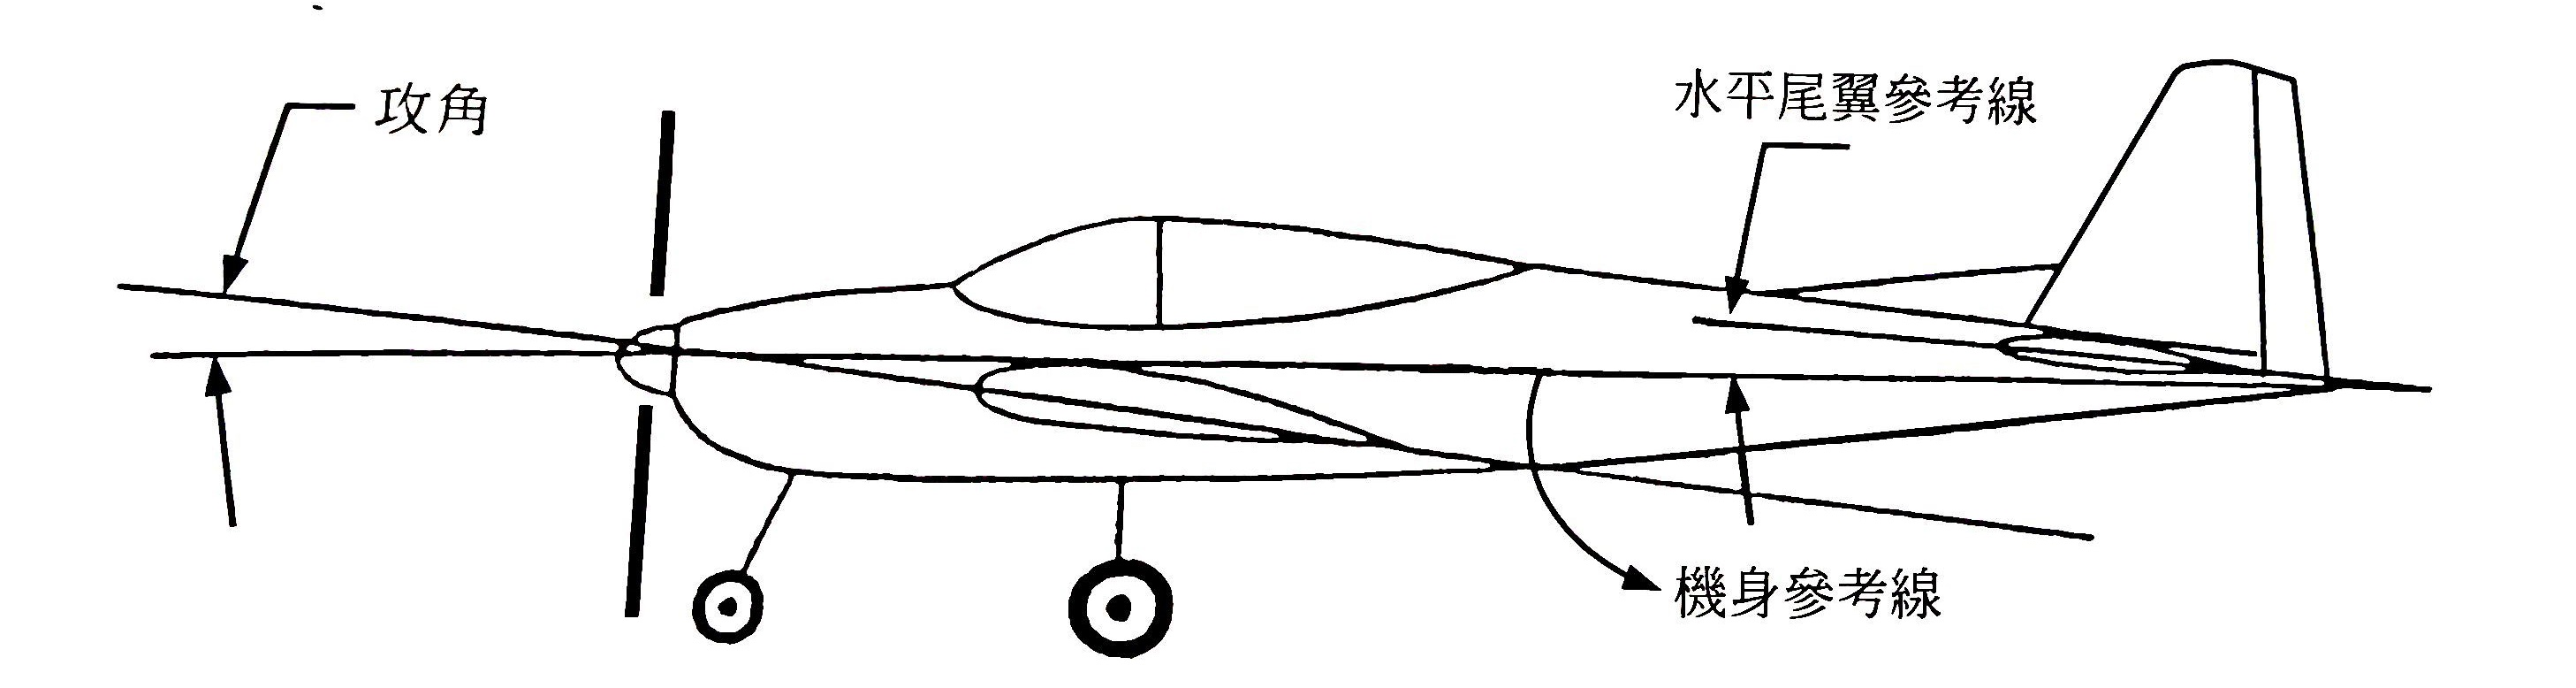
\includegraphics[width=0.7\linewidth]{image/2-3.jpg}
\end{figure}

展弦比(Aspect Ratio):

机翼所能产生的升力的大小取决于其能捕捉或影响到的空气的多少.以相同的翼面积而言,翼展越大所能产生的升力也越大.为了比较翼展(b)和翼面积(S)的相对大小,尝试用一个常数展弦比(Aspect Ratio-AR)来表达:
\begin{equation}
    AR = b^2/S
\end{equation}

如下图所示的几种翼型,对于其中的长方形翼来说,$S = bc$,因此$AR = b^2/bc = b/c$,其分子为翼展,分母为翼弦,这也就是\textbf{展弦比}一名的由来.AR越大者,升力约佳.
\begin{figure}[H]
    \centering
    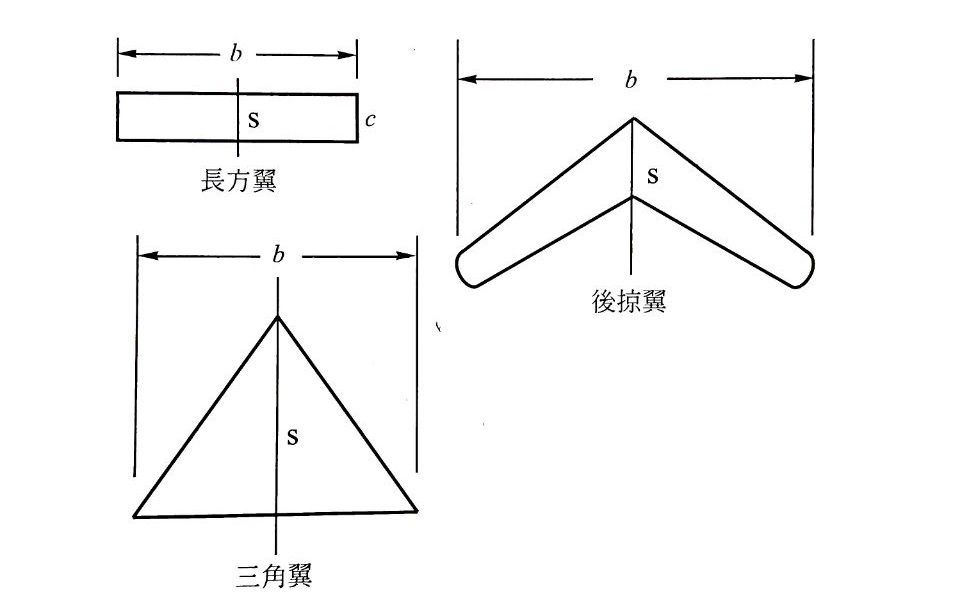
\includegraphics[width=0.6\linewidth]{image/2-4.jpg}
\end{figure}

梯形比(Taper Ratio):

如下图所示,机翼在翼根的弦长$C_r$与在翼尖的弦长$C_t$不一样,两者的比值称为梯形比或跟梢比(名字叫跟梢比,但是实际上是稍比根):
\begin{equation}
    TR = \frac{C_t}{C_r}
\end{equation}
\begin{figure}[H]
    \centering
    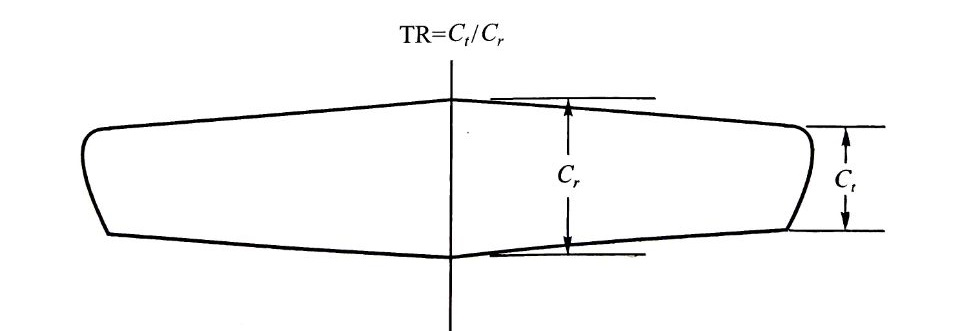
\includegraphics[width=0.6\linewidth]{image/2-5.jpg}
\end{figure}

\section{翼剖面的外型}

机翼的垂直剖面称为翼剖面(airfoil),如下图所示.翼剖面的几何外型,决定翼面所能产生的升力和阻力的大小.
\begin{figure}[H]
    \centering
    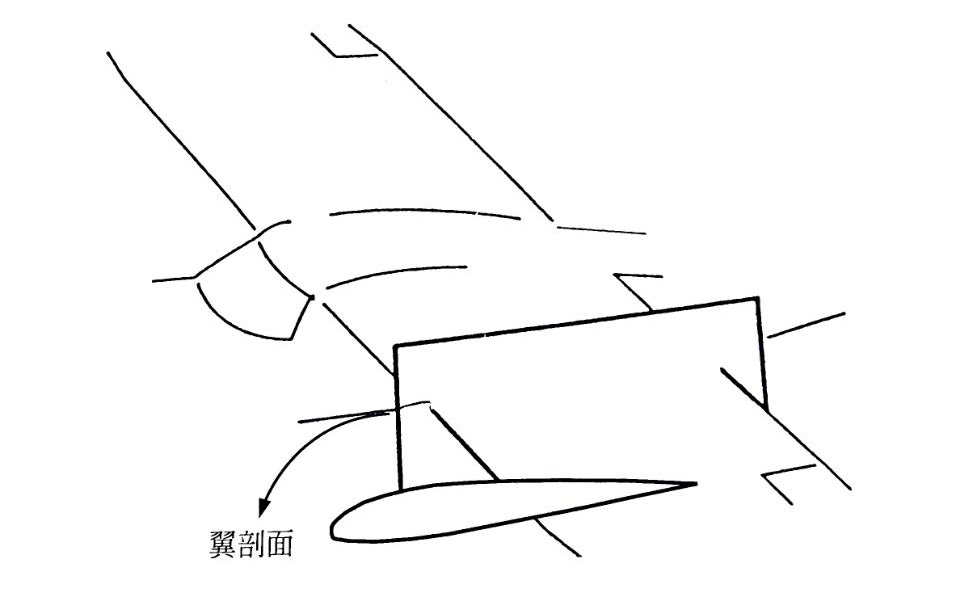
\includegraphics[width=0.6\linewidth]{image/2-6.jpg}
\end{figure}

描述翼剖面的重要物理量包括:
\begin{itemize}
    \item [-] 弦线(Chard Line):连接翼前缘和后缘的直线段.
    \item [-] 中弧线(Mean Camber Line):上下翼面的中点连线\textcolor[rgb]{1,0,0}{(下面图中画的中弧线是这个定义???)}.
    \item [-] 弧高(camber):指弦线和中弧线之间的距离,通常中弧线在弦线的上方(上翼面更长?).对于上下对称的翼面来说,中弧线和弦线重合,故弧高为零.
\end{itemize}

\begin{figure}[H]
    \centering
    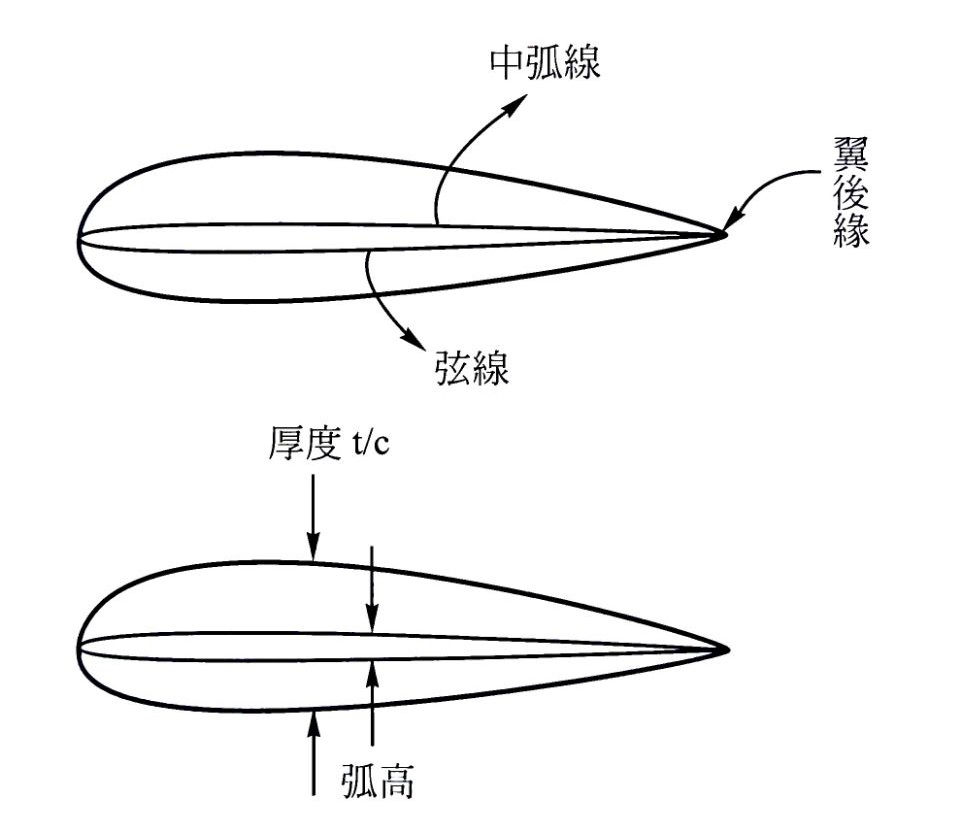
\includegraphics[width=0.5\linewidth]{image/2-7.jpg}
\end{figure}

翼剖面的数字表示法:美国航太总署以4位,5位或6位数字来表示翼剖面的几何外形,如下所示.
\begin{figure}[H]
    \centering
    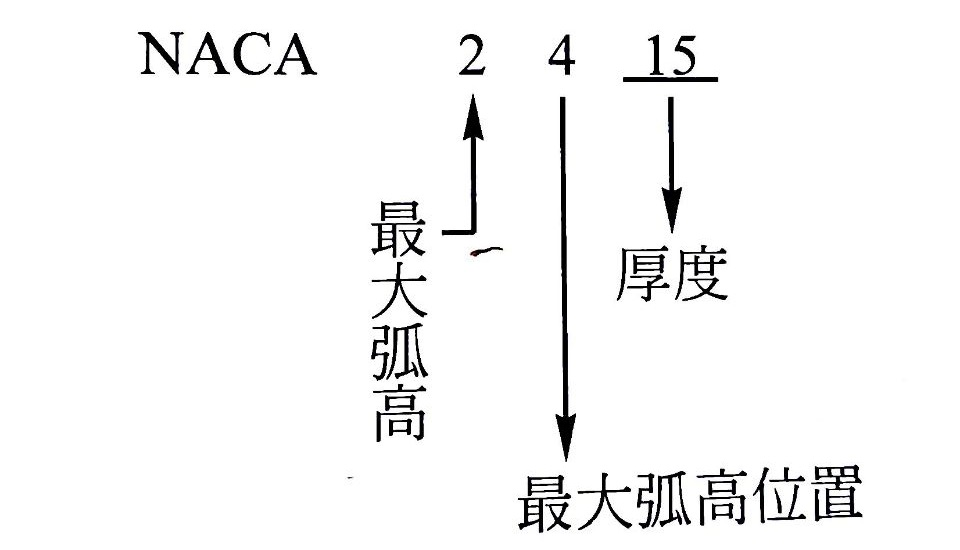
\includegraphics[width=0.3\linewidth]{image/表示法.jpg}
\end{figure}

此四位数字所代表的翼剖面为:

\begin{itemize}
    \item [-] 最大弧高为$2\%$的弦长.
    \item [-] 最大弧高发生的地方距前缘有0.4弦长.
    \item [-] 厚度为$15\%$的弦长.
\end{itemize}

另外,机翼在不同的位置所切的剖面有不同的扭转趋势,例如在翼尖附近的剖面有向下扭转的角度,如下图所示:
\begin{figure}[H]
    \centering
    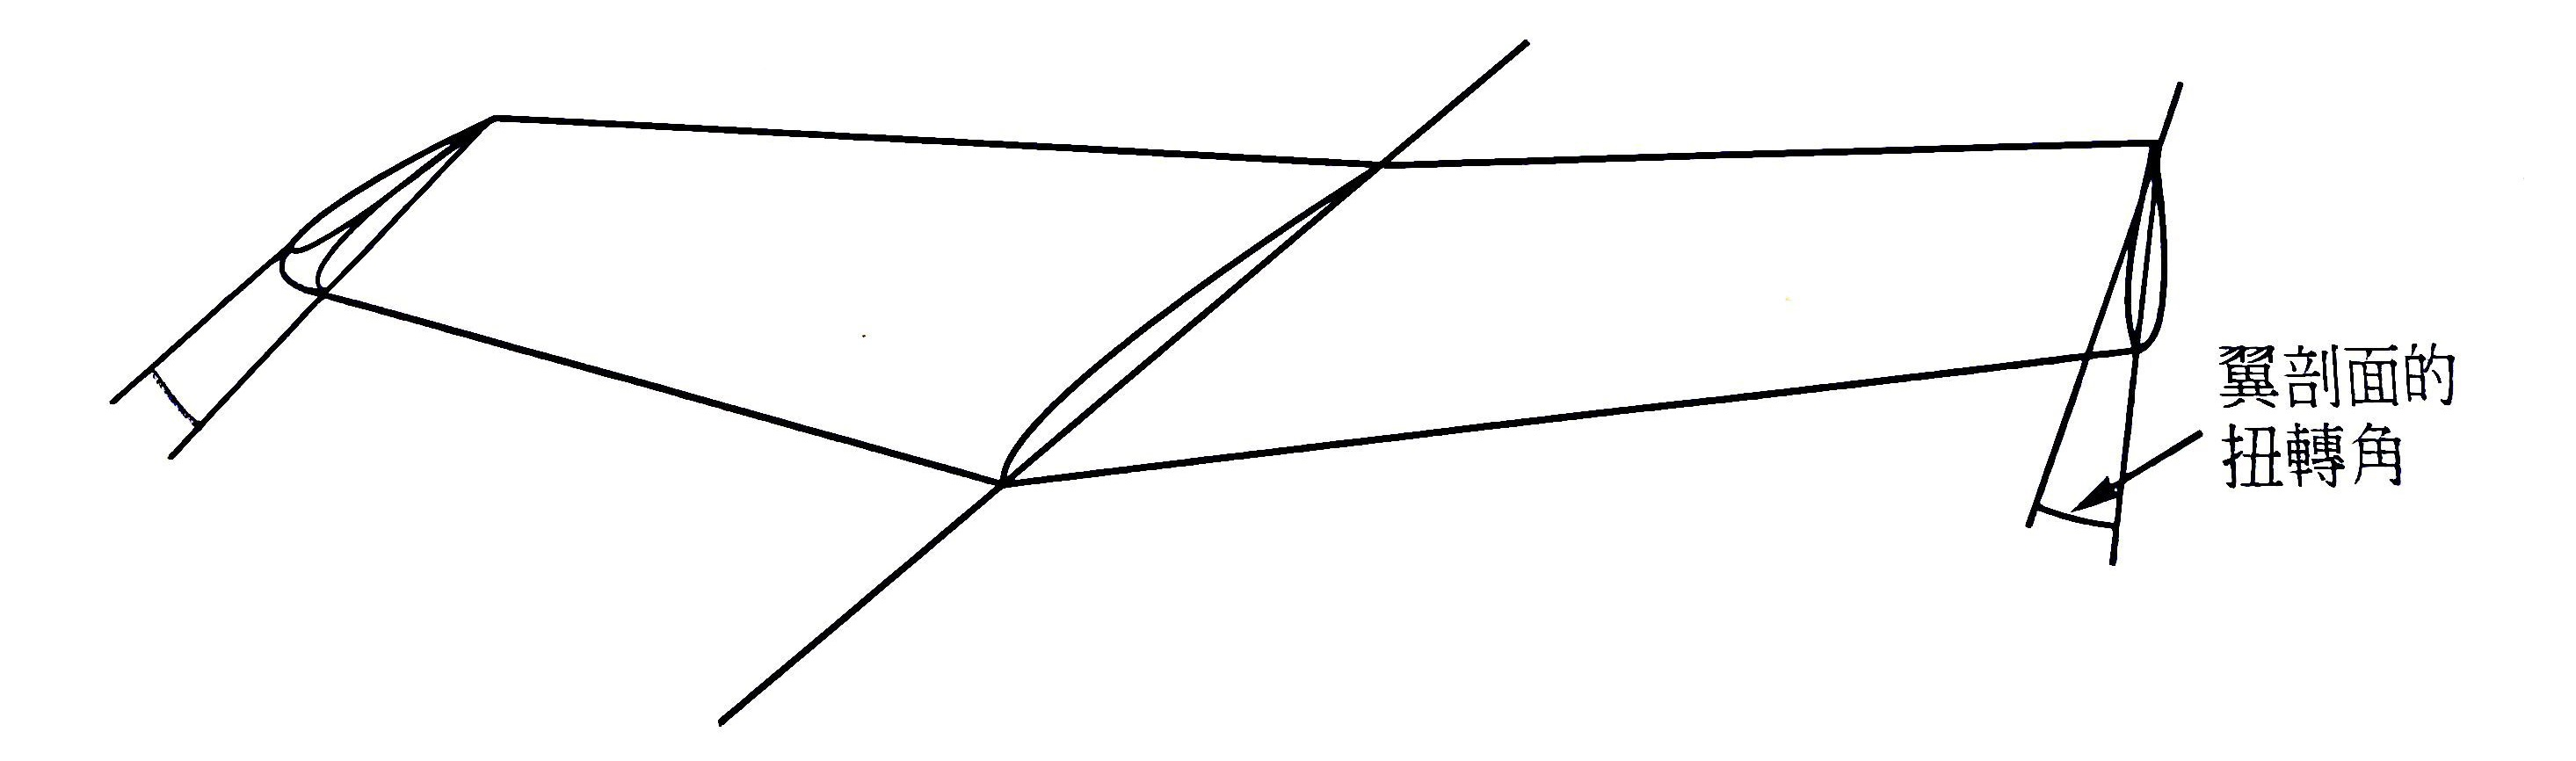
\includegraphics[width=0.6\linewidth]{image/2-8.jpg}
\end{figure}

\section{副翼(aileron)和襟翼(flap)}

副翼是控制面(control surface),襟翼是升力面(lifting surface).如下图所示,副翼在机翼的外缘,用以控制飞机的横滚和偏航动作.左右两个副翼,如果一边打上,则另一边则是打下.襟翼在机翼的内侧,是用以增加翼剖面的弧度或增加翼面的面积,使得升力得以提高.
\begin{figure}[H]
    \centering
    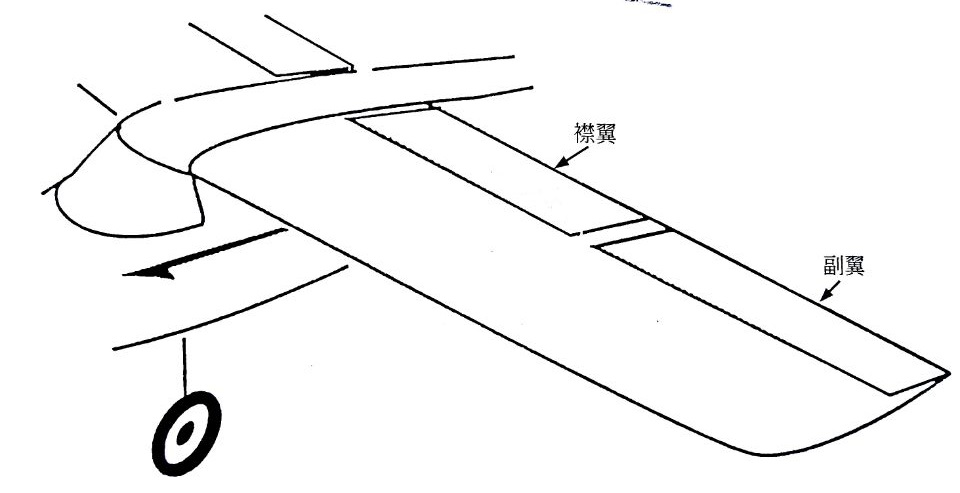
\includegraphics[width=0.6\linewidth]{image/2-9.jpg}
\end{figure}

襟翼有几种不同的型式,如下图所示,其中襟翼延伸得越出去,弧度越大的,其所产生的升力也就越大.
\begin{figure}[H]
    \centering
    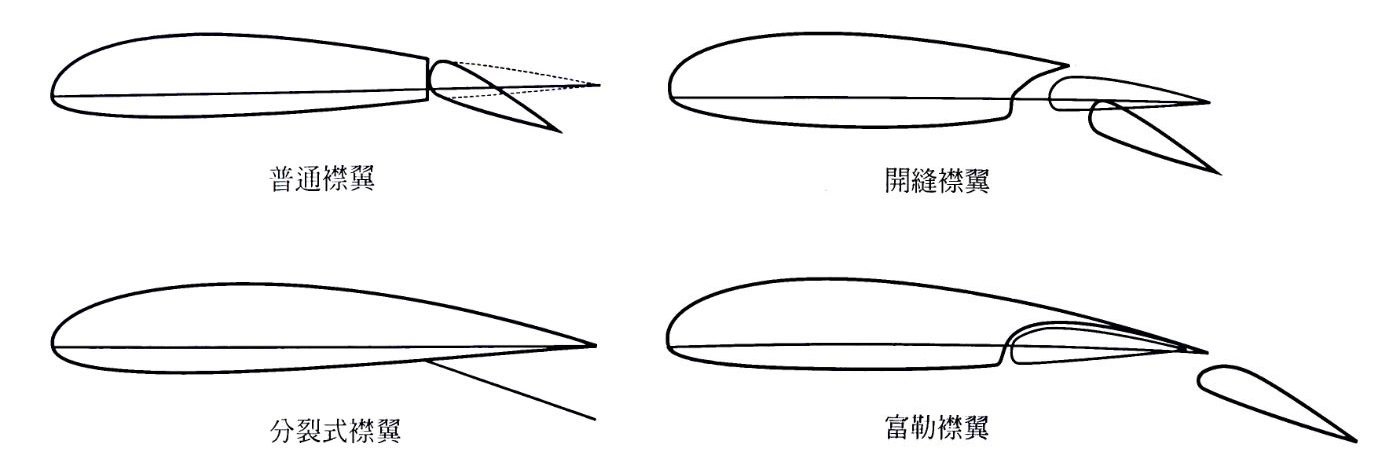
\includegraphics[width=0.8\linewidth]{image/2-10.jpg}
\end{figure}

\section{方向舵(rudder)和升降舵(elevator)}

方向舵(又称为垂直尾舵),是用于飞机水平转向的控制面;升降舵(又称为水平尾舵),是用于改变飞机上升或下降的控制面.通常副翼,方向舵,升降舵统称为控制面(Control Surface),而襟翼则称为升力面(Lifting Surface).

升降舵是水平尾翼的一部分,而水平尾翼先对于机身的位置可能有下面三种情形:在机身上,在垂直尾舵的中间,在垂直尾舵的顶端,如下图所示,各种不同位置均有其优缺点.
\begin{figure}[H]
    \centering
    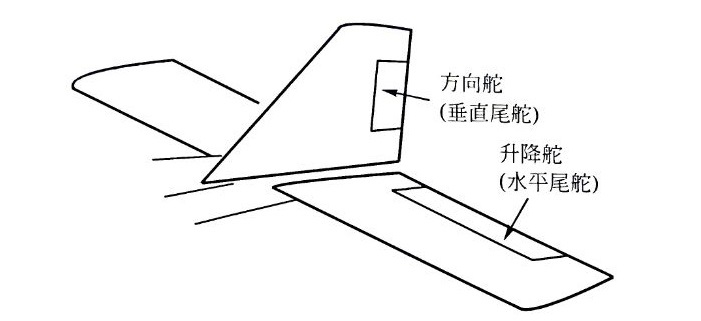
\includegraphics[width=0.5\linewidth]{image/2-11.jpg}
\end{figure}
\begin{figure}[H]
    \centering
    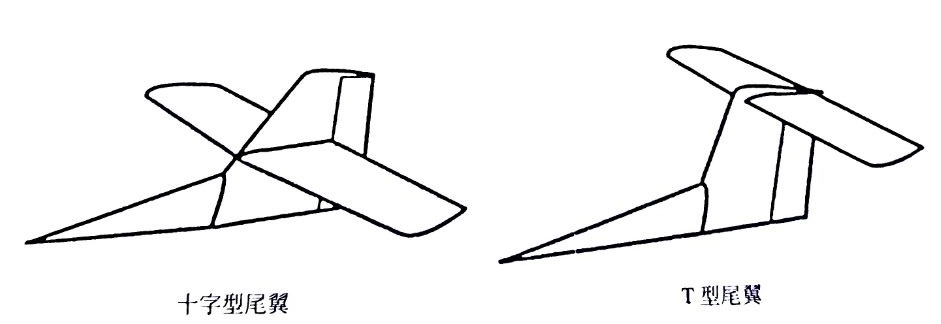
\includegraphics[width=0.6\linewidth]{image/2-12.jpg}
\end{figure}

\section{基本空气动力特性}

\subsection{升力与阻力}

如下图所示,当翼剖面和气流方向有一个夹角的时候,翼面下缘的气流与翼面直接冲击,产生向上的冲击力;而翼面上缘的气流没有受到阻挡,速度加快,从而产生负压区.根据分析,机翼所获得的升力,有2/3来自负压区的作用力,另外1/3来自下缘翼面的空气冲击力.
\begin{figure}[H]
    \centering
    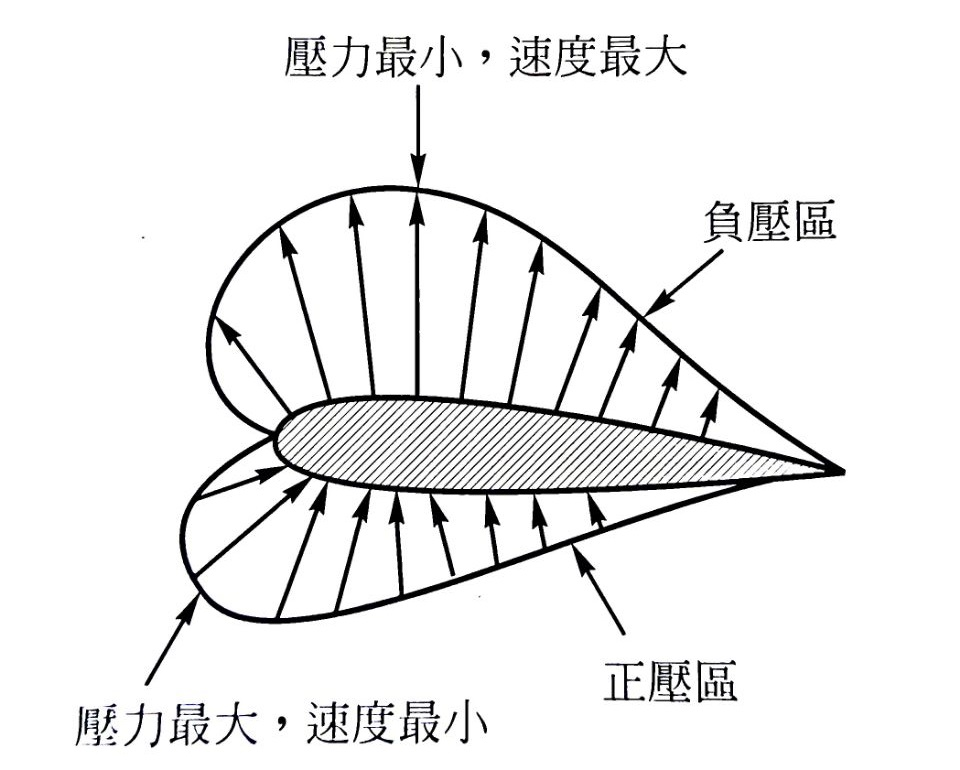
\includegraphics[width=0.35\linewidth]{image/2-13.jpg}
\end{figure}

升力的产生也可以用气流动量的改变来解释.如下图所示,气流从左方水平进来,经过翼面之后,气流被带往右下方.所多出来的向下的气流分量,称为下洗(Down Wash),所产生的合力就是沿着速度变化量$\Delta V_T$的方向.
\begin{figure}[H]
    \centering
    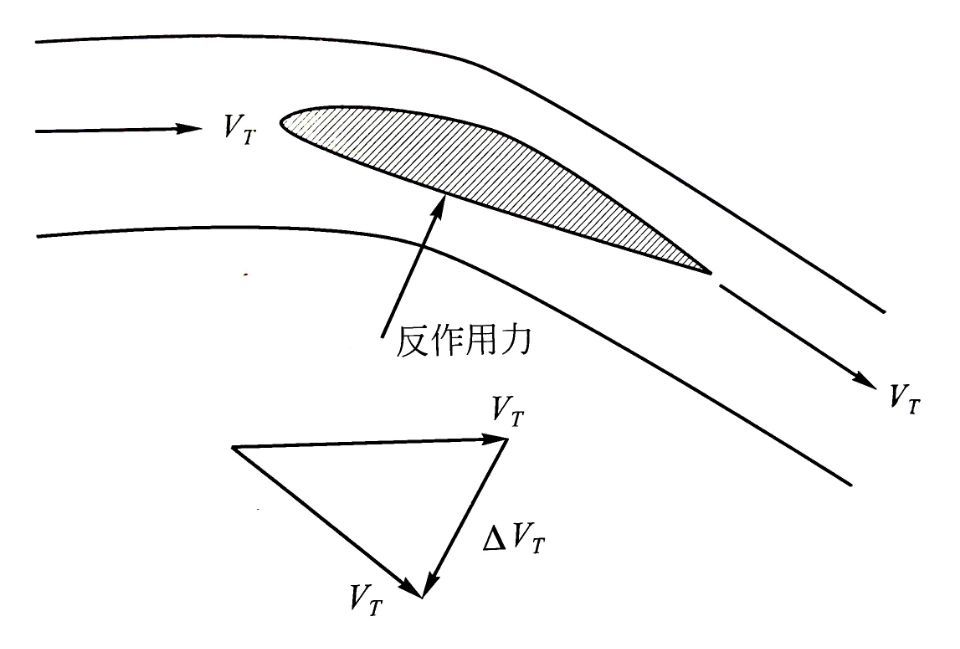
\includegraphics[width=0.4\linewidth]{image/2-14.jpg}
\end{figure}

如下图所示,将气流作用在机翼上的合力拆成两个分量:沿着入射气流方向的为阻力,垂直入射气流方向的为升力.
\begin{figure}[H]
    \centering
    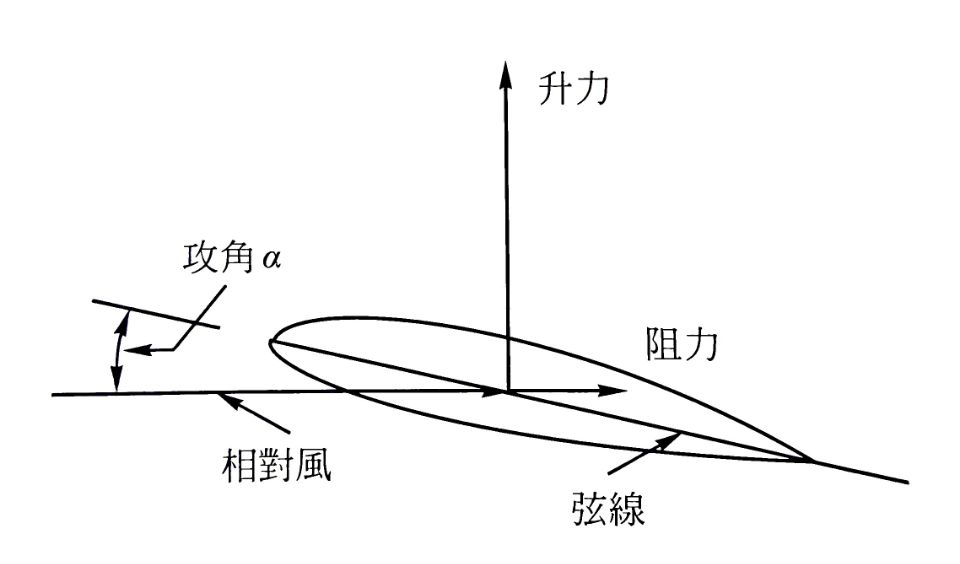
\includegraphics[width=0.5\linewidth]{image/2-15.jpg}
\end{figure}

当攻角越大,上下翼面之间的压力差也就越大,因此可以产生较大的升力.不过当攻角大到某一极限值时,会产生所谓的失速现象,升力不增反降.

当空气以$V_T$的速度冲击到翼面上时,其速度瞬间变为零,由于速度变化所产生的冲击压力称为动压(Dynamic Pressure).如果假设空气不可压缩,则动压可以近似表示为:$Q = 1/2\rho V_T^2$(这就是动压的计算公式),其中$\rho$为飞行器所在高度的大气密度.若将动压乘以翼面的面积,则可以得到冲击力:
\begin{equation}
    \mbox{冲击力} = QS
\end{equation}
    
\subsubsection{升力}

如果定义:
\begin{equation}
    \frac{\mbox{升力}}{\mbox{冲击力}} = \frac{L}{QS} = C_L
\end{equation}

则升力可以表示为:
\begin{equation}
    L = C_LQS
\end{equation}

则我们可以得到影响升力的三个主要因素:

\subparagraph{升力系数$C_L$}:

$C_L$取决于翼剖面的形状,提高翼面的弧度有助于$C_L$的增加,增加翼面的弧度可以利用后缘襟翼(flap)和前缘缝翼(slat).

flap和slat不用时收在主翼之内,在起飞和降落的时候,则延伸出来,以增加飞机的升力.因为在飞机起飞或降落的时候,动压Q很小(速度低),所以只能通过$C_L$来增大L;当飞机起飞后速度提高,动压Q已经足够大,则可以收回flap和slat,同时也可以避免在高速飞行时,襟翼所产生的阻力.

如下图所示,当前后襟翼都收回,升力系数$C_L$最小;伸出后缘襟翼(flap),$C_L$增加;当前后缘襟翼都伸出,升力系数更大.

\begin{figure}[H]
    \centering
    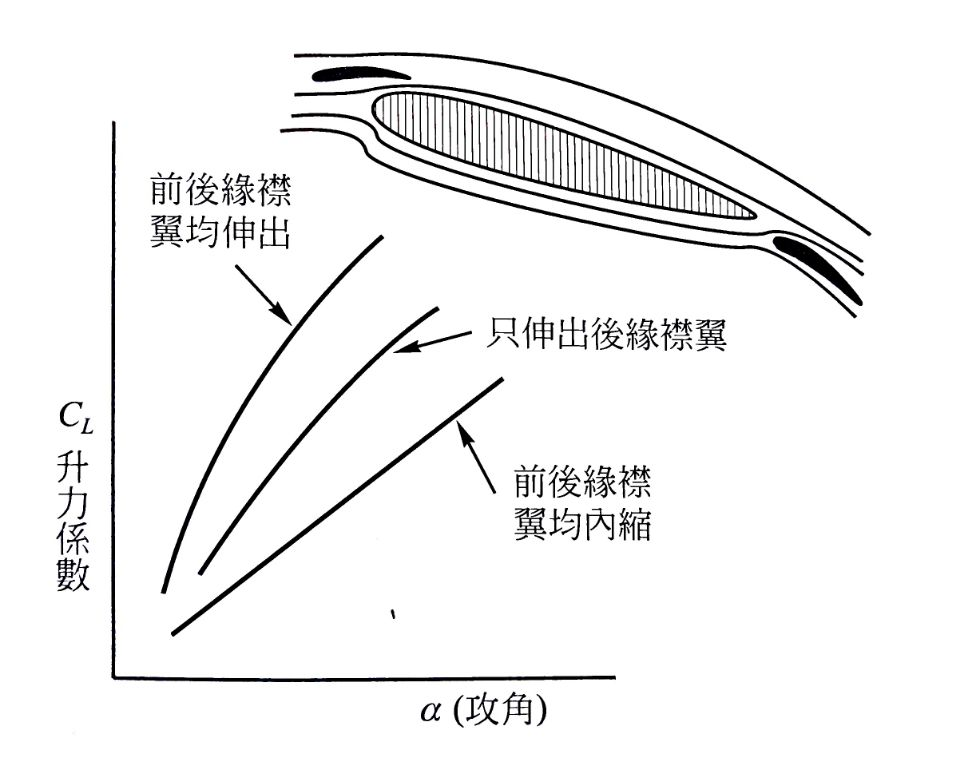
\includegraphics[width=0.4\linewidth]{image/2-16.jpg}
\end{figure}

\subparagraph{动压$Q$}:
$Q = 1/2\rho V_T^2$只是一个近似的公式,在第六章中会推导出更为精确的公式.大的动压的产生,需要有快的速度(大的马赫数M)或大的静气压$P_s$(低空飞行).   

\subparagraph{翼面积S}:
翼面积越大, 升力也呈线性比例增大.比如轻航机,其升力系数$C_L$较小,速度慢则动压$Q$也较小,但是因为其翼面积S足够大,使得它可以飞得像人跑步一样的速度,也不会掉下来.

\subsubsection{阻力}

如果定义:
\begin{equation}
    \frac{\mbox{阻力}}{\mbox{冲击力}} = \frac{D}{QS} = C_D
\end{equation}

则阻力可以表示为:
\begin{equation}
    D = C_DQS
\end{equation}

升力系数和阻力系数之间有如下的近似关系:
\begin{equation}
    C_D = C_{D0} + KC_L^2
\end{equation}

其中$C_{D0}$和$K$为常数,对于不同的翼剖面,这两个常数的值不相同.

已知$C_D$和$C_L$的平方成正比,则当$C_L$小的时候,平方更小;但是当$C_L>1$时,平方会快速增大.\textcolor[rgb]{1,0,0}{(但是升力是冲击力的垂直分力,如果$C_L>1$则升力大于冲击力,会存在这种情况么?)}

如下图所示,对于大部分的攻角而言,$C_D$都很小,只有接近$\alpha_{max}$(当飞机的攻角大于最大攻角时,会产生失速现象)时,$C_D$才会迅速增大.

\begin{figure}[H]
    \centering
    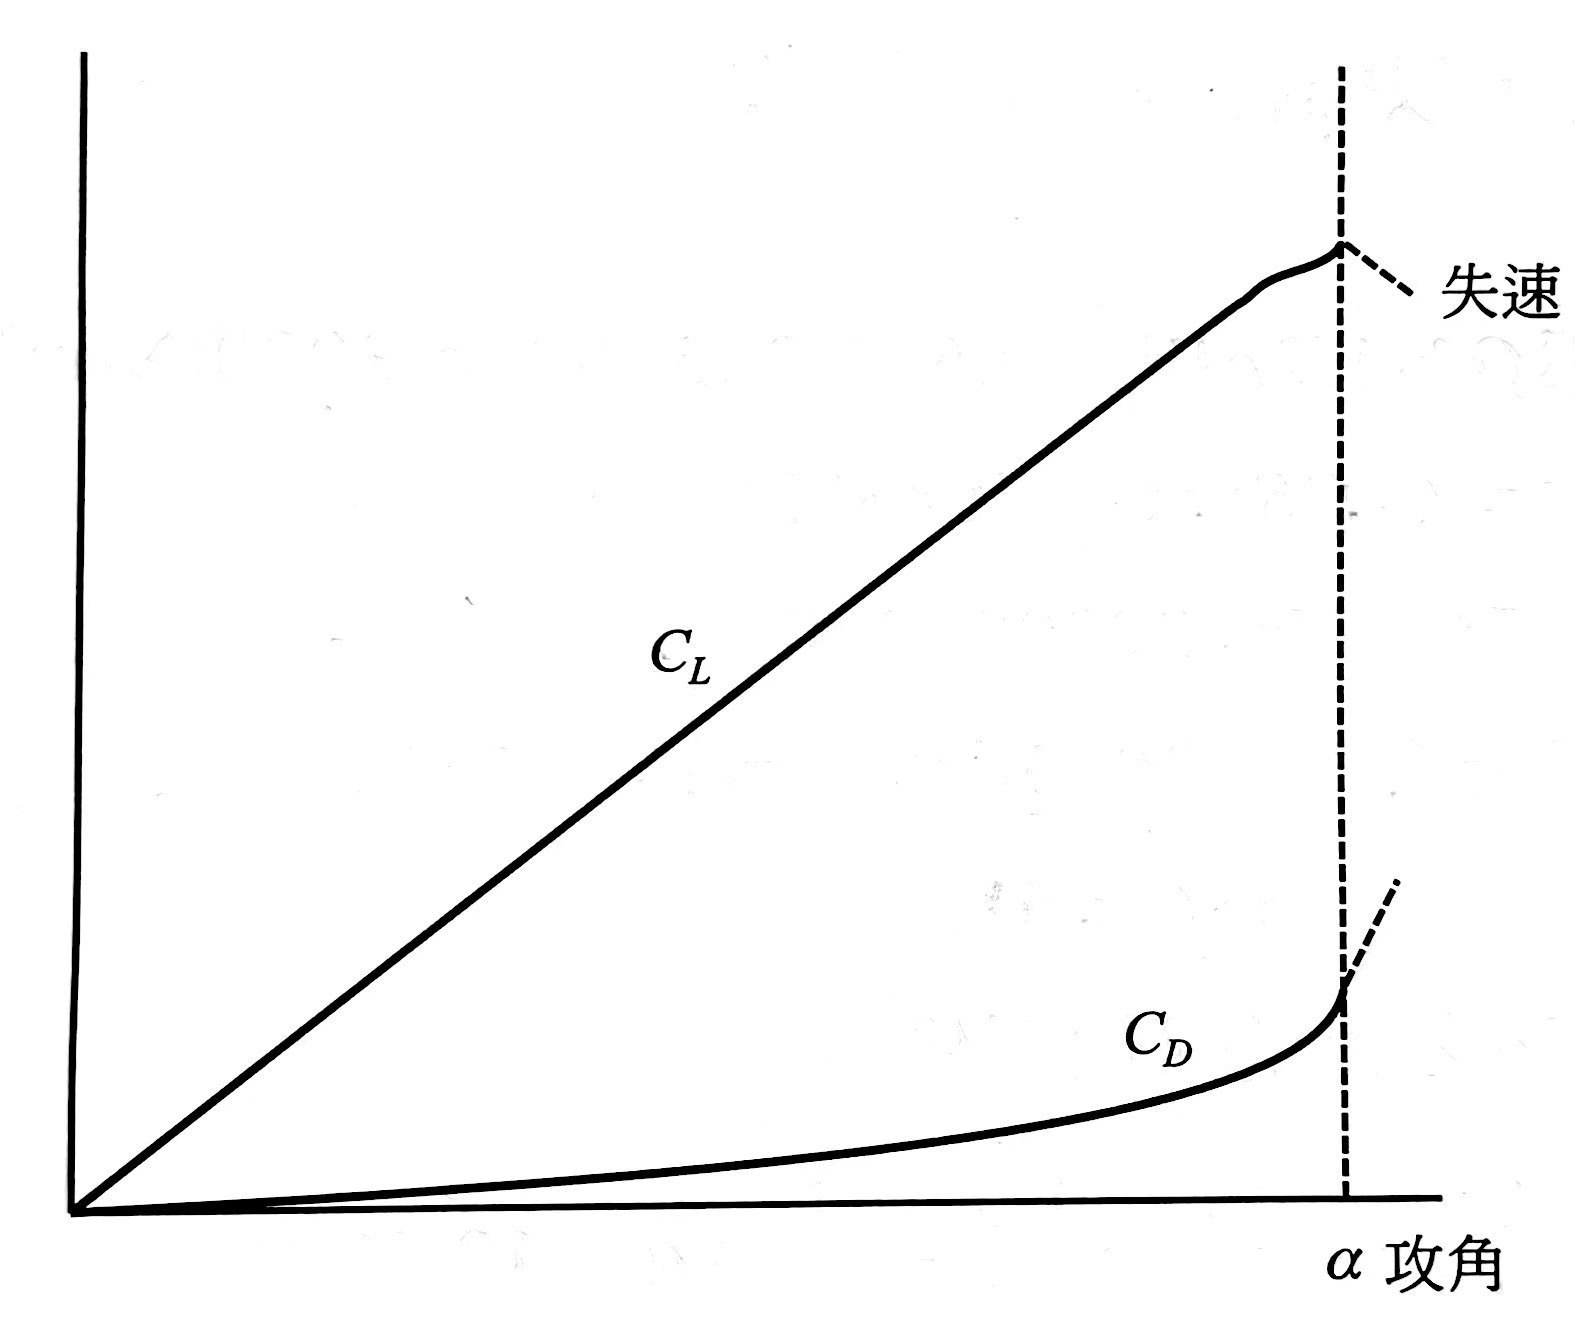
\includegraphics[width=0.4\linewidth]{image/2-17.jpg}
\end{figure}

\subsection{俯仰力矩(pitching moment)}

俯仰力矩一部分由升力造成,另一部分和升力(或攻角)无关.和升力无关的这一部分叫做零升力俯仰力矩(Zero-Lift Pitching Moment),表示如下:
\begin{equation}
    M_0 = 1/2\rho V_T^2C_{M0}Sc
\end{equation}

其中c表示平均弦长,约等于$S/b$(b为翼展),因为及以上不同位置的翼剖面,其弦长也不同,故取平均弦长.


当机身俯仰到某一个角度,要保持静止时,可以使用水平尾翼达到一个平衡的状态,如下图所示,机翼所产生的升力和阻力假设集中于空气动力中心(Aerodynamic Center).

\begin{figure}[H]
    \centering
    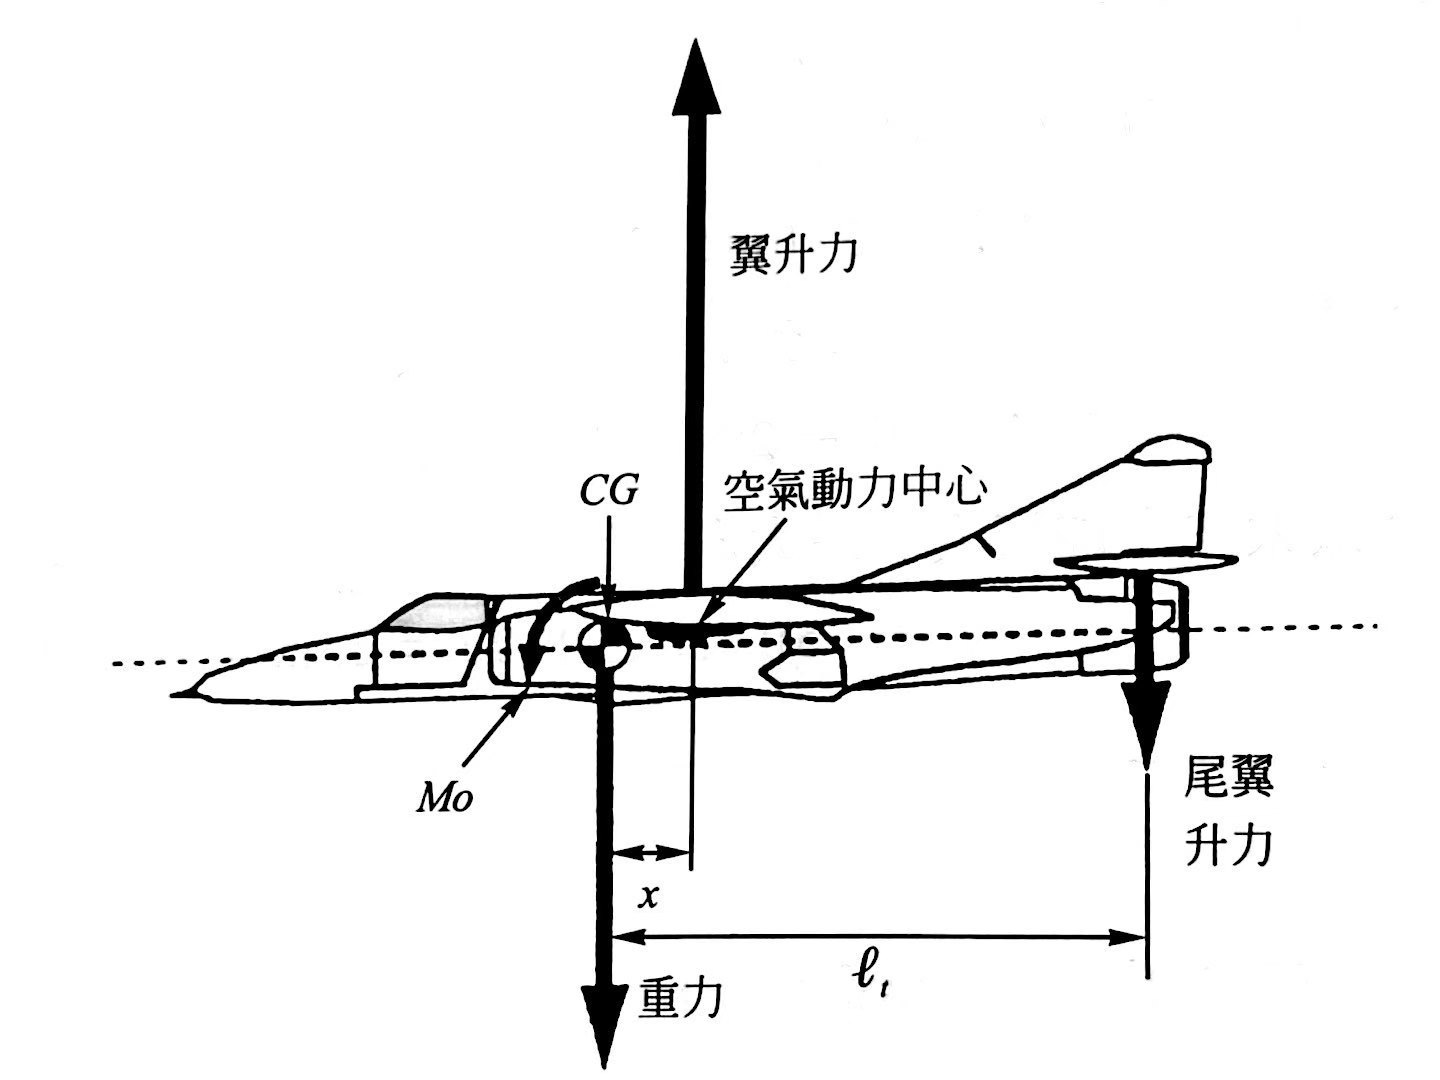
\includegraphics[width=0.5\linewidth]{image/2-18.jpg}
\end{figure}

假设使机头上仰的力矩为正,则作用在重心$c.g.$上的力矩可表示为:
\begin{equation}
    M = -L_Wx - M_0 + L_tl_t
\end{equation}

其中零升力俯仰力矩$M_0$和主翼伤力$L_W$使机头下俯,而水平尾翼升力$L_t$使机头上仰,故而可以形成平衡.

不过因为水平尾翼的升力是向下的,而主翼的升力是向上的,使得主翼的升力有一部分被水平尾翼的升力抵消掉了,这是稳定飞机的缺点.

公式推导:
\begin{equation}
    \mbox{主翼升力:} L_W = 1/2\rho V_T^2SC_L
\end{equation}
\begin{equation}
    \mbox{零升力俯仰力矩:} M_0 = 1/2\rho V_T^2ScC_{M0}
\end{equation}
\begin{equation}
    \mbox{水平尾翼升力:} L_t = K_t1/2\rho V_T^2S_tC_{Lt}
\end{equation}

其中$S_t$为水平尾翼的面积,$C_{Lt}$为水平尾翼的升力系数,$K_t$水平尾翼的效率因子.
\begin{equation}
    K_t = \frac{\mbox{水平尾翼附近的动压}}{\mbox{自由流的动压}}
\end{equation}

水平尾翼附近的气流场系受到主翼下洗(Down Wash)气流的影响,故其动压和自由流动压不同,$K_t$的值约介于$0.65\sim 0.95$之间.

水平尾翼对重心$c.g.$所产生的力矩为:
\begin{equation}
    L_tl_t = K_t1/2\rho V_T^2C_{Lt}S_tl_t
\end{equation}

其中,$S_tl_t$称为水平尾翼的体积(Tailplane Volume),此体积越大,代表水平尾翼对飞行俯仰运动的影响越大.

将作用在重心$c.g.$上的力矩表达式展开,两边除以$1/2\rho V_T^2Sc$,得到:
\begin{equation}
    C_M = -\frac{x}{c}C_L - C_{M0} + K_t\frac{S_tl_t}{Sc}C_{Lt}
\end{equation}

其中,$C_M$称为总俯仰力矩系数,包含三个组成项:

\bm{$-\frac{x}{c}C_L$}:是因主翼升力所产生的力矩.

\bm{$-C_{M0}$}:是零升力(零攻角)之下,主翼所具有的俯仰力矩.

\bm{$K_t\frac{S_tl_t}{Sc}C_{Lt}$}:是因水平尾翼所造成的力矩.

我们将


























\end{document}